\documentclass[tikz,border=1mm]{standalone}
\usepackage{amsmath,amssymb,fontspec,unicode-math}
\setmainfont{STIXTwoText-Regular.otf}
\setmathfont{STIXTwoMath-Regular.otf}
\usetikzlibrary{arrows.meta,calc}
% Diagram of a representation, not a new HMT generating construction.
% Sources: REV04 manuscript, spin block at lines 4363--4373;
% Integral2249, 04ac_geometria_proyectiva_bloch_rev2.tex,
% equations coordenadas-bloch-rev2, proyector-bloch-rev2,
% fibrado-hopf-bloch-rev2.
\begin{document}
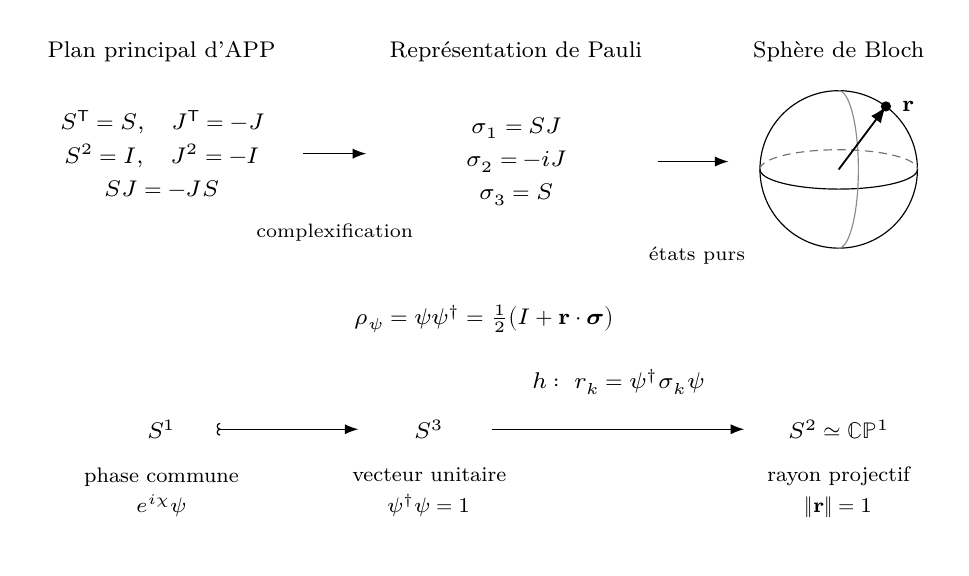
\begin{tikzpicture}[x=1mm,y=1mm,>=Latex,
  font=\fontsize{8.2}{10}\selectfont,
  every node/.style={inner sep=0pt},
  line width=.42pt]
\path[use as bounding box] (0,-61) rectangle (116,5);

\node[align=center] at (17,2) {Plan principal d’APP};
\node[align=center] at (17,-11)
  {$S^{\mathsf T}=S,\quad J^{\mathsf T}=-J$\\[2pt]
   $S^2=I,\quad J^2=-I$\\[2pt]$SJ=-JS$};
\draw[->] (35,-11)--(43,-11);
\node[font=\fontsize{7}{8.5}\selectfont,align=center] at (39,-21)
  {complexification};

\node[align=center] at (62,2) {Représentation de Pauli};
\node[align=center] at (62,-12)
  {$\sigma_1=SJ$\\[2pt]$\sigma_2=-iJ$\\[2pt]$\sigma_3=S$};
\draw[->] (80,-12)--(89,-12);
\node[font=\fontsize{7}{8.5}\selectfont,align=center] at (85,-24)
  {états purs};

\node[align=center] at (103,2) {Sphère de Bloch};
\draw (103,-13) circle (10);
\draw[densely dashed,black!55] (93,-13) arc[start angle=180,end angle=0,x radius=10,y radius=2.5];
\draw (93,-13) arc[start angle=180,end angle=360,x radius=10,y radius=2.5];
\draw[black!45] (103,-23) arc[start angle=-90,end angle=90,x radius=2.5,y radius=10];
\draw[->,line width=.65pt] (103,-13)--(109,-5);
\fill (109,-5) circle (.65);
\node[anchor=west] at (111,-5) {$\symbf r$};

\node at (58,-32)
  {$\rho_\psi=\psi\psi^\dagger=\tfrac12\bigl(I+\symbf r\cdot\symbf\sigma\bigr)$};

\node at (17,-46) {$S^1$};
\draw[Hooks-Latex] (24,-46)--(42,-46);
\node at (51,-46) {$S^3$};
\draw[->] (59,-46)--(91,-46);
\node at (75,-40) {$h:\ r_k=\psi^\dagger\sigma_k\psi$};
\node at (103,-46) {$S^2\simeq\mathbb{CP}^{1}$};
\node[font=\fontsize{7.6}{9}\selectfont,align=center] at (17,-54)
  {phase commune\\[2pt]$e^{i\chi}\psi$};
\node[font=\fontsize{7.6}{9}\selectfont,align=center] at (51,-54)
  {vecteur unitaire\\[2pt]$\psi^\dagger\psi=1$};
\node[font=\fontsize{7.6}{9}\selectfont,align=center] at (103,-54)
  {rayon projectif\\[2pt]$\|\symbf r\|=1$};
\end{tikzpicture}
\end{document}
